\section{temp}
\subsection{Visitor Pattern}
\begin{frame}{Traversing the Tree}
\framesubtitle{Visitor Pattern}
	\begin{itemize}
        \item ANTLR visitor pattern
        \item Our own Visitor Pattern
    \end{itemize}
    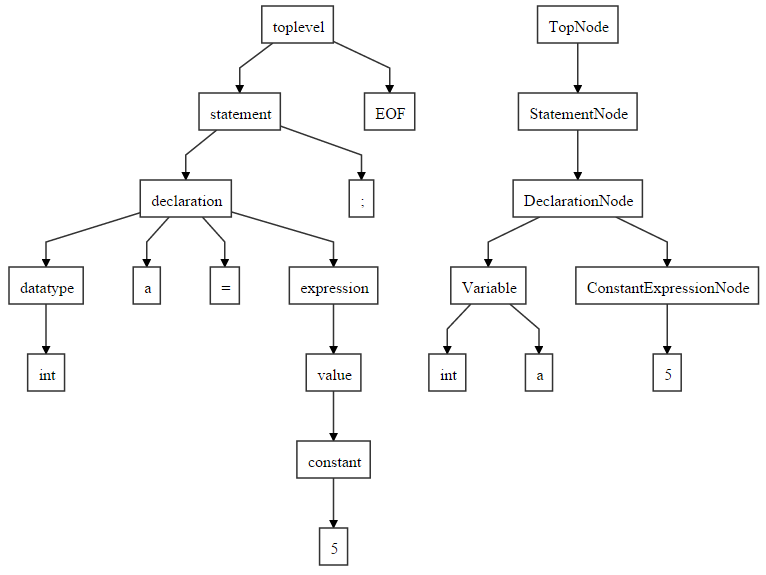
\includegraphics[width=1\textwidth,height=0.7\textheight,keepaspectratio, , clip]{images/P4/AST.PNG}

\end{frame}

\begin{frame}[fragile]{Contextual Analysis}
\framesubtitle{Module call}

    \begin{lstlisting}[caption=The creation of an instance of the Contextual analysis module and the call invoking it. ,frame=tlrb, basicstyle=\tiny, numbers=none]
ContextualAnalyser contextualAnalyser = 
 new ContextualAnalyser(inputFile, errors);

abstractSyntaxTree = 
 contextualAnalyser.GenerateDecoratedASTFromParseTree(abstractSyntaxTree);
    \end{lstlisting}


\end{frame}

\subsection{Contextual Analysis}
\begin{frame}[fragile]{Contextual Analysis}

\framesubtitle{The Module}

\begin{lstlisting}[caption=The method called from main performing Scope and Type checking and also reporting errors. ,frame=tlrb, basicstyle=\tiny, numbers=none ]
public BaseASTNode GenerateDecoratedASTFromParseTree(BaseASTNode abstractSyntaxTree){

  //Add potential imported function declarations
  handleImports(abstractSyntaxTree);

  //Scope check
  SymbolTable symbolTable = new SymbolTable();
  scopeCheck(abstractSyntaxTree, symbolTable);
  //Type check
  typeCheck(abstractSyntaxTree, symbolTable);

  //Check for unused variables
  errors.addAll(symbolTable.getUnusedVariables());

  //Error Handling
  ErrorReporter errorReporter = new ErrorReporter();
  errorReporter.HandleErrors(errors, ErrorType.ALL);

  return abstractSyntaxTree;
}
\end{lstlisting}
\end{frame}

\subsubsection{Scope Checking}
\begin{frame}[fragile]{Scope Checking}
\framesubtitle{Creating Variables}


\begin{lstlisting}[caption=The visit method for visiting a DeclarationNode in the Scope checker. ,frame=tlrb, basicstyle=\tiny, numbers=none]
@Override
public Void VisitDeclarationNode(DeclarationNode node) {
  Symbol tmpSym = symbolTable.currentScope().resolve(node.getVariable().getId());
  if (tmpSym != null) {
    errors.add(new ReDeclarationError(node.getVariable(), tmpSym, symbolTable.currentScope(), node.getLineNumber()));
  } else {
      node.setScope(symbolTable.currentScope());
      symbolTable.currentScope().define(node.getVariable(), node.getLineNumber());
  }
  if (node.getVariable().isComplex() && node.getVariable().getDynamicSize() != null){
    visit(node.getVariable().getDynamicSize()[0]);
    visit(node.getVariable().getDynamicSize()[1]);
  }
  return super.VisitDeclarationNode(node);
}
\end{lstlisting}

\end{frame}

\subsubsection{Type Checking}
\begin{frame}[fragile]{Type Checking}
\framesubtitle{Using Expressions}


\begin{lstlisting}[caption=The visit method for visiting a ExpressionNode in the Type checker. ,frame=tlrb, basicstyle=\tiny, numbers=none]
@Override
public Variable VisitExpressionNode(ExpressionNode node) {
  ValueType valueType = TypeChecker.CombineValueTypes(
    node.getLValue() != null ? visit(node.getLValue()) : null,
    node.getRValue() != null ? visit(node.getRValue()) : null,
    errors,
    node.getLineNumber()
  );

  node.setValueType(valueType);

  if (TypeParser.isComplexValueType(valueType) && node.getOperatorType() != null && !OperatorType.isAllowed(node.getOperatorType())){
    System.out.println("\nOperator not allowed at the moment!\n");
    System.exit(1);
  }

  return new Variable(valueType, "Expr:<" + node.toString() + ">");
}
\end{lstlisting}

\end{frame}

\begin{frame}[fragile]{Type Checking}
\framesubtitle{Using Expressions}

\begin{lstlisting}[caption=The method checking if two types are compatible according to the specification of GAMBL ,frame=tlrb, basicstyle=\tiny, numbers=none]
public static ValueType CombineValueTypes(Variable lValue, Variable rValue, ArrayList<LanguageError> errors, int lineNum) {
  if (lValue == null) {
    return ValueType.INVALID;
  } else if (rValue == null) {
      return lValue.getValueType();
  } else {
    if (rValue.isFunction() && rValue.getId().equals("fileToMatrix"))
    return lValue.getValueType();
    
  ValueType combined = compatibleTypes(
    lValue.getEntrance() != null ? ComplexToSimple(lValue.getValueType()) : lValue.getValueType(),
    rValue.getEntrance() != null ? ComplexToSimple(rValue.getValueType()) : rValue.getValueType());
  if (combined != ValueType.INVALID) {
    return combined;
  } else {
      errors.add(new TypeMismatchError(lValue, rValue, lineNum));
      return ValueType.INVALID;
    }
  }
}
\end{lstlisting}

\end{frame}

\subsection{Code Generation}
\begin{frame}[fragile]{Code Generation}
\framesubtitle{Module Call}

\begin{lstlisting}[caption=The creation of an instance of the Code Generation module and the call invoking it ,frame=tlrb, basicstyle=\tiny, numbers=none]
CodeGenerator codeGenerator = new CodeGenerator();
codeGenerator.GenerateCodeAndWriteToFile(abstractSyntaxTree);
\end{lstlisting}

\end{frame}

\begin{frame}[fragile]{Code Generation}
\framesubtitle{The Module Method}

\begin{lstlisting}[caption=The method called from main performing Code Generation and exporting the files generated along with the needed libraries.,frame=tlrb, basicstyle=\tiny, numbers=none]
public void GenerateCodeAndWriteToFile(BaseASTNode abstractSyntaxTree){
  FileHandling filesNstuff = new FileHandling();
  StringBuilder output = new StringBuilder();

  abstractSyntaxTree.accept(new CodeGeneratorVisitor(output));

  filesNstuff.WriteToFile(
    filesNstuff.GetFileForOutputCode("code.c", "codeout/"),
    output);

  filesNstuff.ExportResource("simpleCL.h", "codeout/");
  filesNstuff.ExportResource("simpleCL.c", "codeout/");
  filesNstuff.ExportResource("complexTypes.h", "codeout/");
  filesNstuff.ExportResource("Makefile", "codeout/");
  filesNstuff.ExportResource("gambleStdlib.c", "codeout/");
  filesNstuff.ExportResource("gambleStdlib.h", "codeout/");
}

\end{lstlisting}

\end{frame}

\begin{frame}[fragile]{Code Generation}
\framesubtitle{Generating the For loop}

\begin{lstlisting}[caption=The visit method called generating code for the for loop.,frame=tlrb, basicstyle=\tiny, numbers=none]
@Override
public String VisitForLoopNode(ForLoopNode node) {
  StringBuilder forLoop = new StringBuilder();
  forLoop.append("for(");
  if (node.getInitialize() != null)
    forLoop.append(visit(node.getInitialize()) + " ");
  else
    forLoop.append("; ");
  if (node.getCondition() != null)
   forLoop.append(visit(node.getCondition()));
  forLoop.append("; ");
  if (node.getUpdate() != null)
    forLoop.append(visit(node.getUpdate()));
  forLoop.append(") {\n");
  forLoop.append(statementBody(node.getBody().getChildren()));
  forLoop.append(indent("}\n"));

  return forLoop.toString();
}

\end{lstlisting}

\end{frame}

\begin{frame}[fragile]{Code Generation}
\framesubtitle{Template for entry checking}
\begin{lstlisting}[caption=The template for checking if an entry is out of bounds in a matrix.,frame=tlrb, basicstyle=\tiny, numbers=none]
if(\S ROW \S < \S MATRIX\S .rows && \S COL\S < \S MATRIX\S.cols){
  \S CODE\S
} else {
  printf("\nTrying to access entry out of bounds in %s\n", " \S MATRIX\S ");
  exit(0);
}

\end{lstlisting}

\end{frame}


\begin{frame}[fragile]{Code Generation}
\framesubtitle{Replacing in the template}
\begin{lstlisting}[caption=The visit method called generating code for the for loop.,frame=tlrb, basicstyle=\tiny, numbers=none]
@Override
private String applyBoundsCheck(Variable variable, String code){
  return filesNstuff.ImportStringFromResource("codesnippets/matrixOutOfBounds.c")
    .replaceAll("\S ROW\S", visit(variable.getEntrance().getCoordinates()[0]))
    .replaceAll("\S COL\S ",
      variable.getEntrance().getCoordinates()[1] != null ?
      visit(variable.getEntrance().getCoordinates()[1]) :
      "0")
    .replaceAll("\S MATRIX\S ", variable.getId())
    .replaceAll("\S CODE\S ", code)
    .replaceAll("\\n", "\n" + indent(""));
}

\end{lstlisting}

\end{frame}







